\section{Strategy Taxonomy}
\label{app:taxonomy}

The six mechanism-level categories that constrain plan declarations:

\begin{table}[h]
  \centering\small
  \begin{tabular}{lp{9.5cm}}
    \toprule
    Category & Mechanism \\
    \midrule
    \texttt{confrontation} & External action toward the threat (fight, challenge, resist) \\
    \texttt{self\_empowerment} & Internal transformation (grow stronger, gain abilities) \\
    \texttt{safety} & Environment modification (safe spaces, protective elements) \\
    \texttt{cognitive\_reframe} & Meaning change (reinterpret threatening elements) \\
    \texttt{social\_support} & Adding allies (introduce helpful figures) \\
    \texttt{sensory\_modulation} & Sensory and calming details (modify light, sound, texture; introduce comforting elements) \\
    \bottomrule
  \end{tabular}
  \caption{Final strategy taxonomy (v4).}
\end{table}

The taxonomy evolved over four iterations ($8 \to 6 \to 7 \to 6$ categories). The initial version suffered a severe skew: a broad empowerment/mastery category absorbed 87.7\% of all picks. Merging it made the skew worse (100\% dominance of a single ``agency'' category). The resolution was a mechanism-level split distinguishing external action (\texttt{confrontation}) from internal transformation (\texttt{self\_empowerment}). A seventh category (\texttt{emotional\_regulation}) was merged into \texttt{sensory\_modulation} after smoke testing showed it was picked in 0.4\% of trials. Category definitions describe \emph{how} the dream changes (mechanism), not what the change achieves (outcome), with NOT-examples to reduce overlap.

\section{Prompts}
\label{app:prompts}

The fused-generation system prompt injected into each trial (the \texttt{\{categories\_block\}} placeholder is filled with the six taxonomy definitions of Appendix~\ref{app:taxonomy}):

\begin{quote}\small\ttfamily\raggedright
You are an Imagery Rehearsal Therapy (IRT) assistant helping a patient rescript their nightmare.\\[2pt]
First, select 1-2 therapeutic strategies from this taxonomy:\\
\{categories\_block\}\\[2pt]
Choose the strategies most specifically suited to THIS patient's nightmare content. Avoid defaulting to general approaches when a more specific mechanism fits.\\[2pt]
Then respond to the patient using those strategies.\\[2pt]
STRICT output format:\\
Line 1: <plan>category1 / category2</plan>\\
Line 2: (empty)\\
Line 3+: Your therapeutic response (conversational, supportive, max 3 sentences)\\[2pt]
IMPORTANT:\\
- You MUST include the closing </plan> tag on the SAME line as the opening tag.\\
- The <plan> line must contain ONLY category names, nothing else.\\
- Do NOT put your response inside the <plan> tags.
\end{quote}

An in-context example provided with the prompt:

\begin{quote}\small\ttfamily\raggedright
<plan>safety / social\_support</plan>\\[4pt]
What if, in this version of the dream, you could find a place that feels completely secure --- and someone you trust is already there waiting for you?
\end{quote}

Each trial receives this system prompt together with the frozen dialogue history (slice~2 of the vignette's generated session), so all trials of a condition share byte-identical input.

\section{Judge Rubric}
\label{app:judge}

The alignment judge receives the taxonomy definitions, the trial's declared strategies, and the therapist response, and scores each declared strategy on a ternary scale with mandatory reasoning:

\begin{quote}\small\ttfamily\raggedright
For each declared strategy, assign ONE score:\\
- 2 (implemented): The response clearly and specifically implements this strategy. The therapeutic technique is evident and developed --- you can point to specific sentences or passages that demonstrate it.\\
- 1 (partial): The response touches on this strategy but does not fully develop it. Elements are present but incomplete, only implied, or mentioned without therapeutic depth.\\
- 0 (absent): The response does not implement this strategy. No evidence of this technique in the response.\\[2pt]
Output format: strategy\_id: <reasoning> | score: <0|1|2>
\end{quote}

Per-trial alignment is the mean score over declared strategies, normalised by the maximum (2). Trials whose judgment fails (timeout, API error) or that cannot be judged (invalid plan) are treated as missing data and excluded from the alignment mean. Zero-scored or partially parsed judgments are re-judged once by Gemini~3.1~Pro (9 of 7{,}200 trials; Section~\ref{sec:results-alignment}).

Because the judge runs at $T{=}1.0$ and scores each trial once, a re-judging control quantifies its own sampling variance: one seeded trial per run (360 trials) was re-judged with the identical setup. Strategy-level exact agreement is 96.2\% (720 score pairs, linear-weighted $\kappa = 0.807$), 93.1\% of trials keep their alignment value unchanged, and the mean signed difference is $-0.003$. Disagreement concentrates in the partial category (score 1), while full implementation (score 2) reproduces at 98.2\%. Single judgments are therefore noisy at the implemented--partial boundary but not biased.

\clearpage

\section{Plan Validity}
\label{app:validity}

Figure~\ref{fig:validity} reports the plan validity rate per model, the upstream quality gate for Method~1.

\begin{figure}[h]
  \centering
  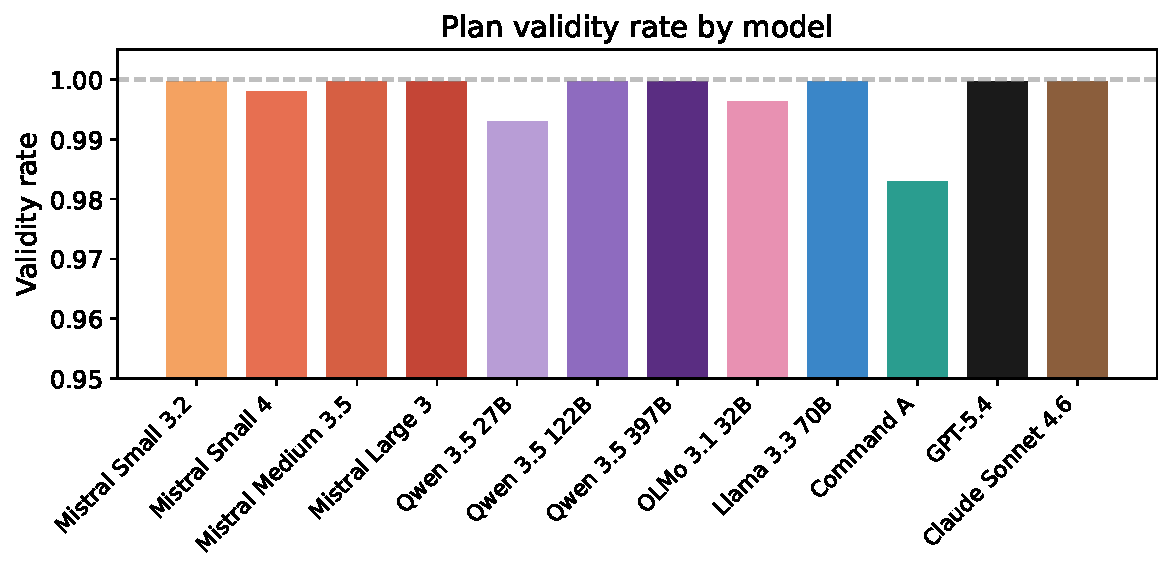
\includegraphics[width=.85\linewidth]{fig_A1_validity}
  \caption{Plan validity rate by model: fraction of trials whose \texttt{<plan>} block parses to valid taxonomy categories.}
  \label{fig:validity}
\end{figure}

\section{Modal-Set Agreement}
\label{app:modal}

Figure~\ref{fig:modal} complements the pairwise Jaccard analysis with modal-set agreement, the fraction of trials whose declared strategy set equals the run's most common set (Section~\ref{sec:results-jaccard}).

\begin{figure}[H]
  \centering
  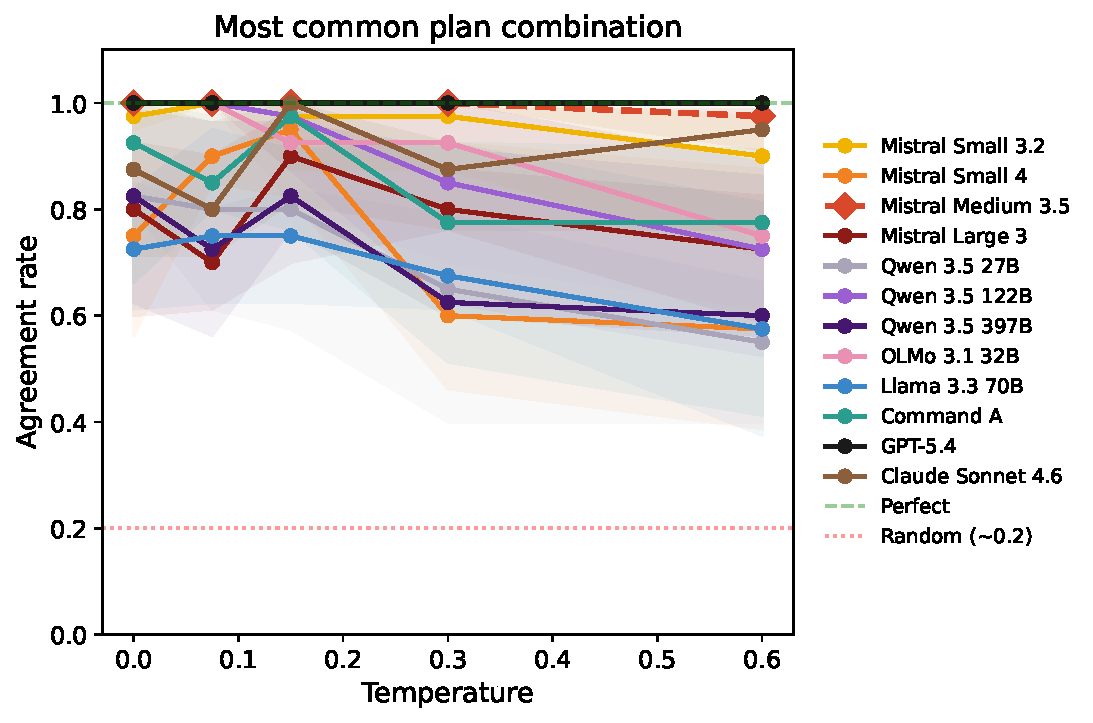
\includegraphics[width=.73\linewidth]{fig_5_2b_modal_agreement}
  \caption{Modal-set agreement by model and temperature: fraction of trials whose declared strategy set equals the run's modal set.}
  \label{fig:modal}
\end{figure}

\clearpage

\section{Per-Vignette Stability}
\label{app:vignettes}

Figure~\ref{fig:vignettes} breaks decision consistency down to individual model--vignette cells, one heatmap per temperature, for consultation of specific combinations.

\begin{figure}[H]
  \centering
  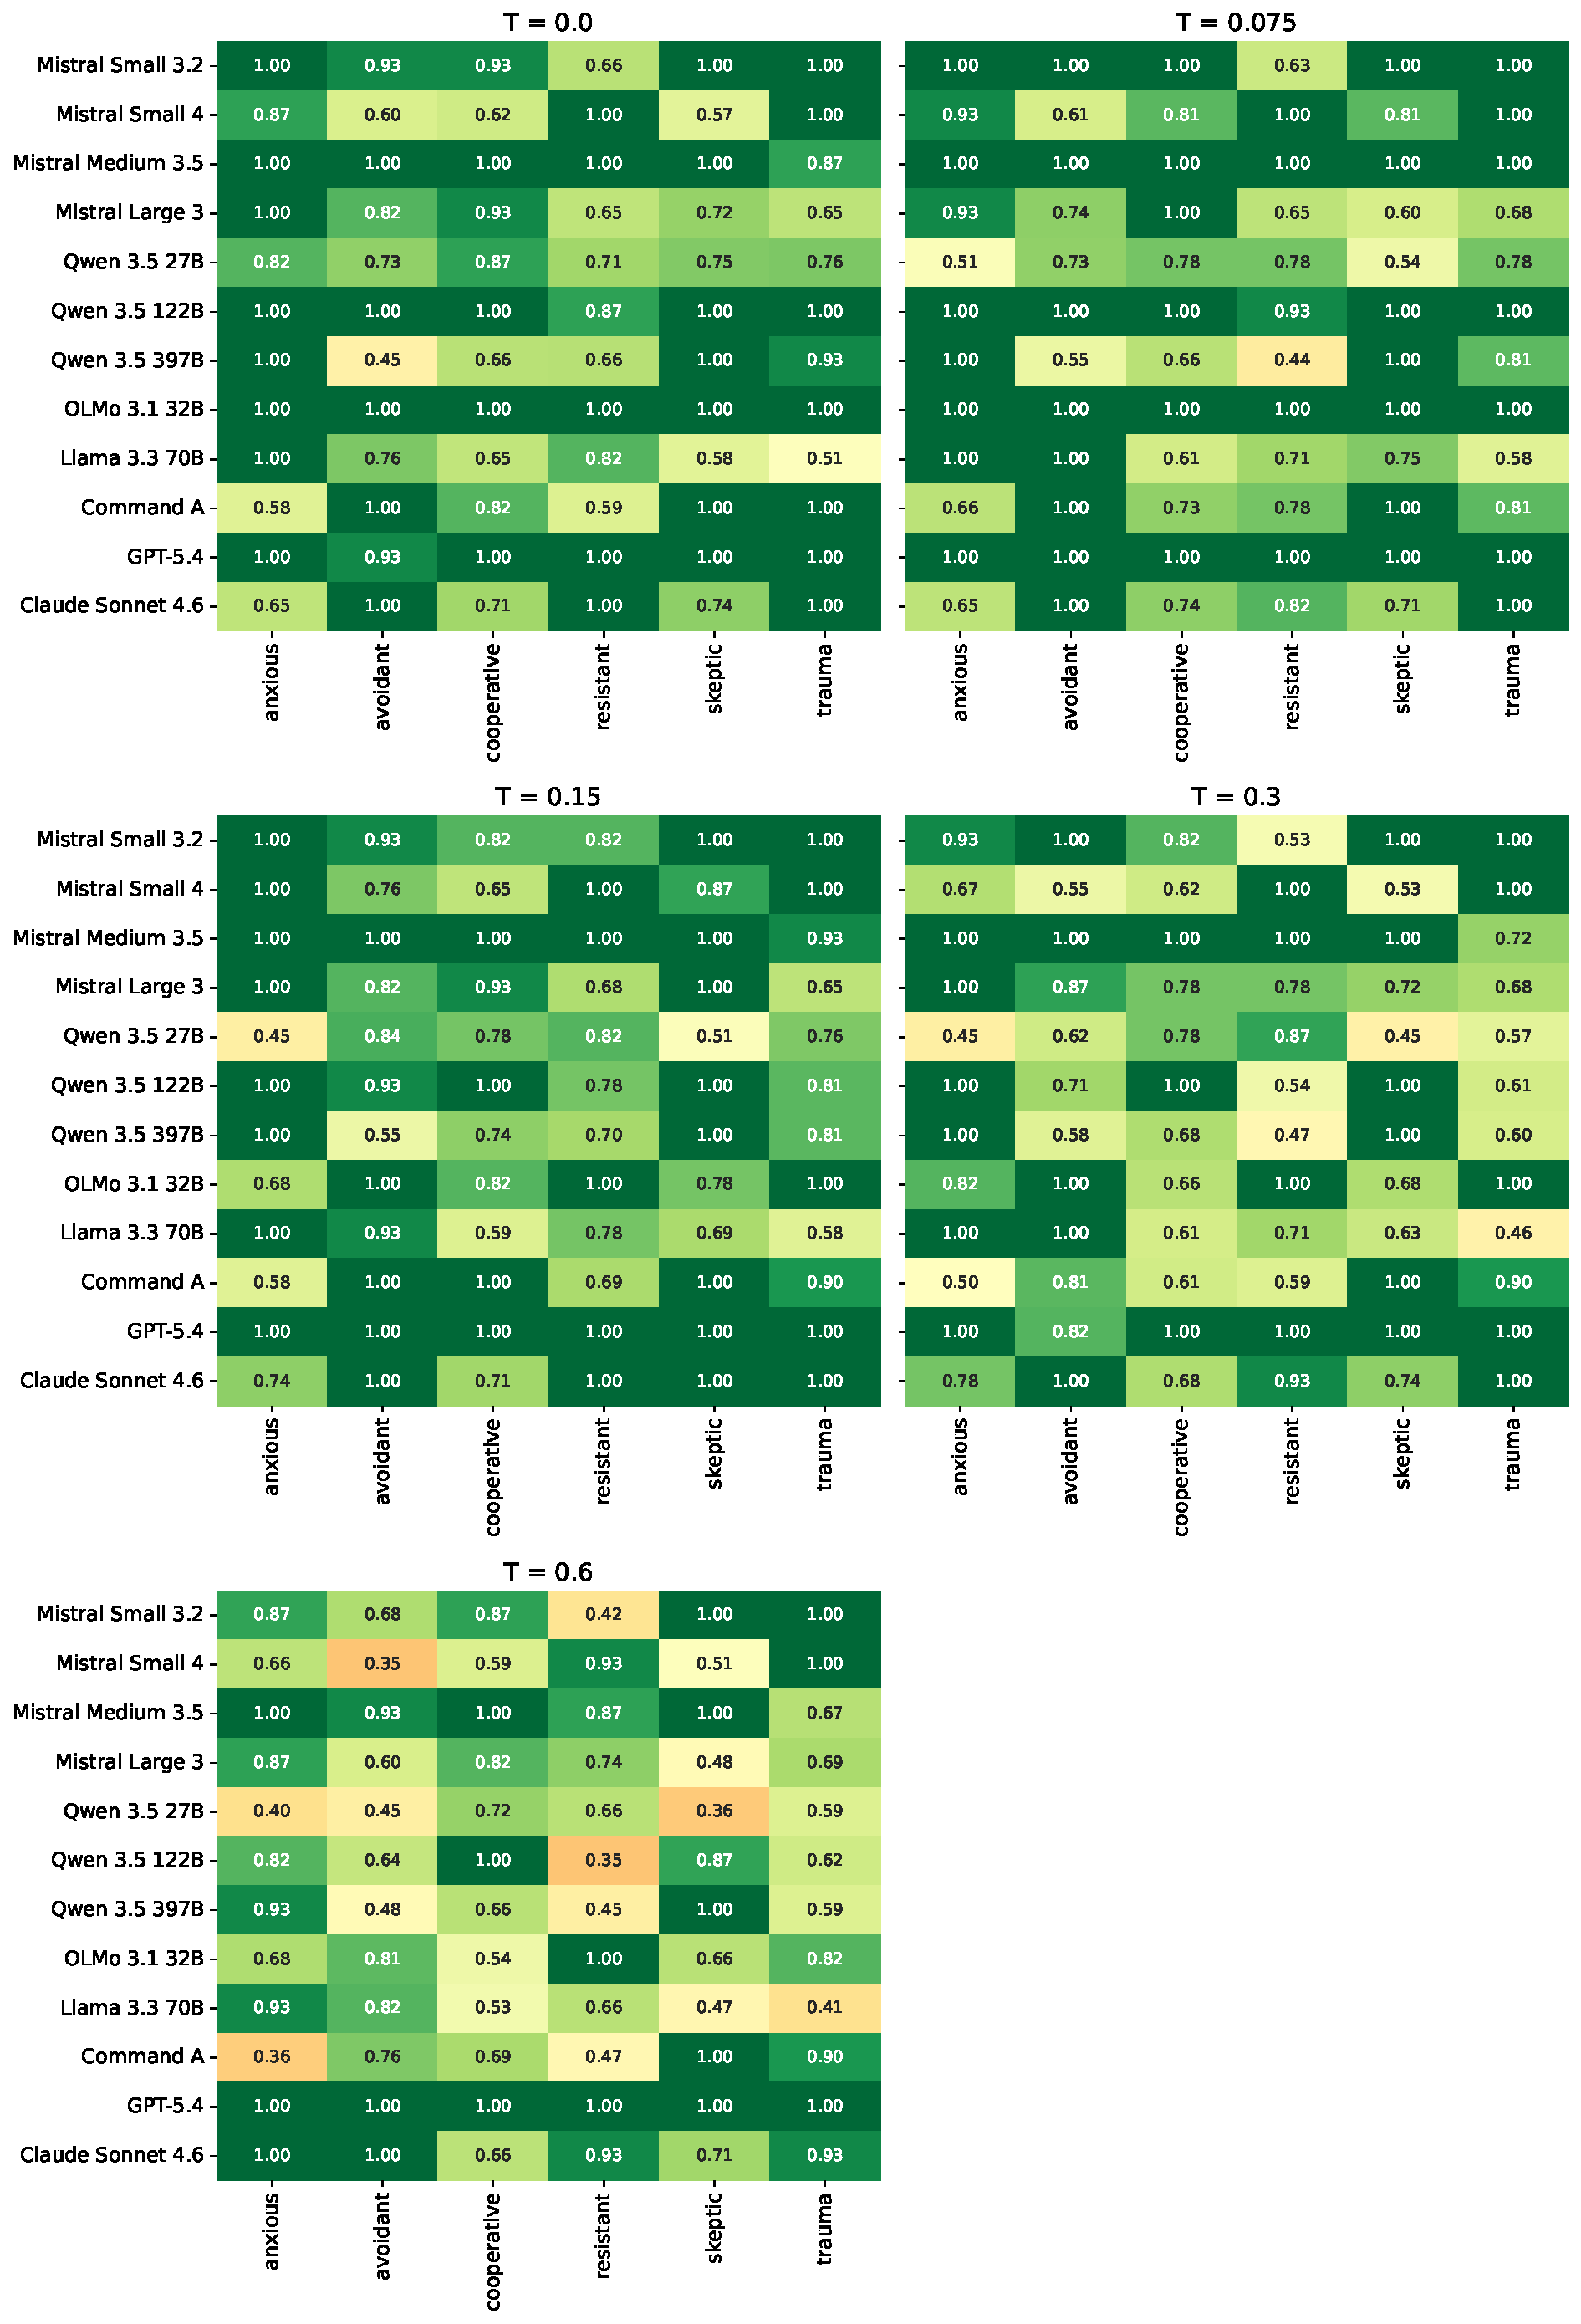
\includegraphics[width=\linewidth,height=.8\textheight,keepaspectratio]{fig_5_4_vignette_slice}
  \caption{Median Jaccard per model $\times$ vignette, one heatmap per temperature. Individual model--vignette combinations can deviate noticeably from the aggregate even though the overall vignette effect is not significant (Section~\ref{sec:results-vignettes}).}
  \label{fig:vignettes}
\end{figure}

\clearpage

\section{Seed Control Experiment}
\label{app:seed}

A supplementary experiment on Mistral Large~3 compares runs with a fixed seed (\texttt{seed=42}) against unseeded runs under otherwise identical conditions. Fixing the seed does not improve consistency (Figure~\ref{fig:seed}): vendor seed support is best effort at most, and residual serving-side nondeterminism persists \citep{yuan2025understanding}. The main experiment therefore sets no seed and captures stochastic variance through trial repetition instead.

\begin{figure}[h]
  \centering
  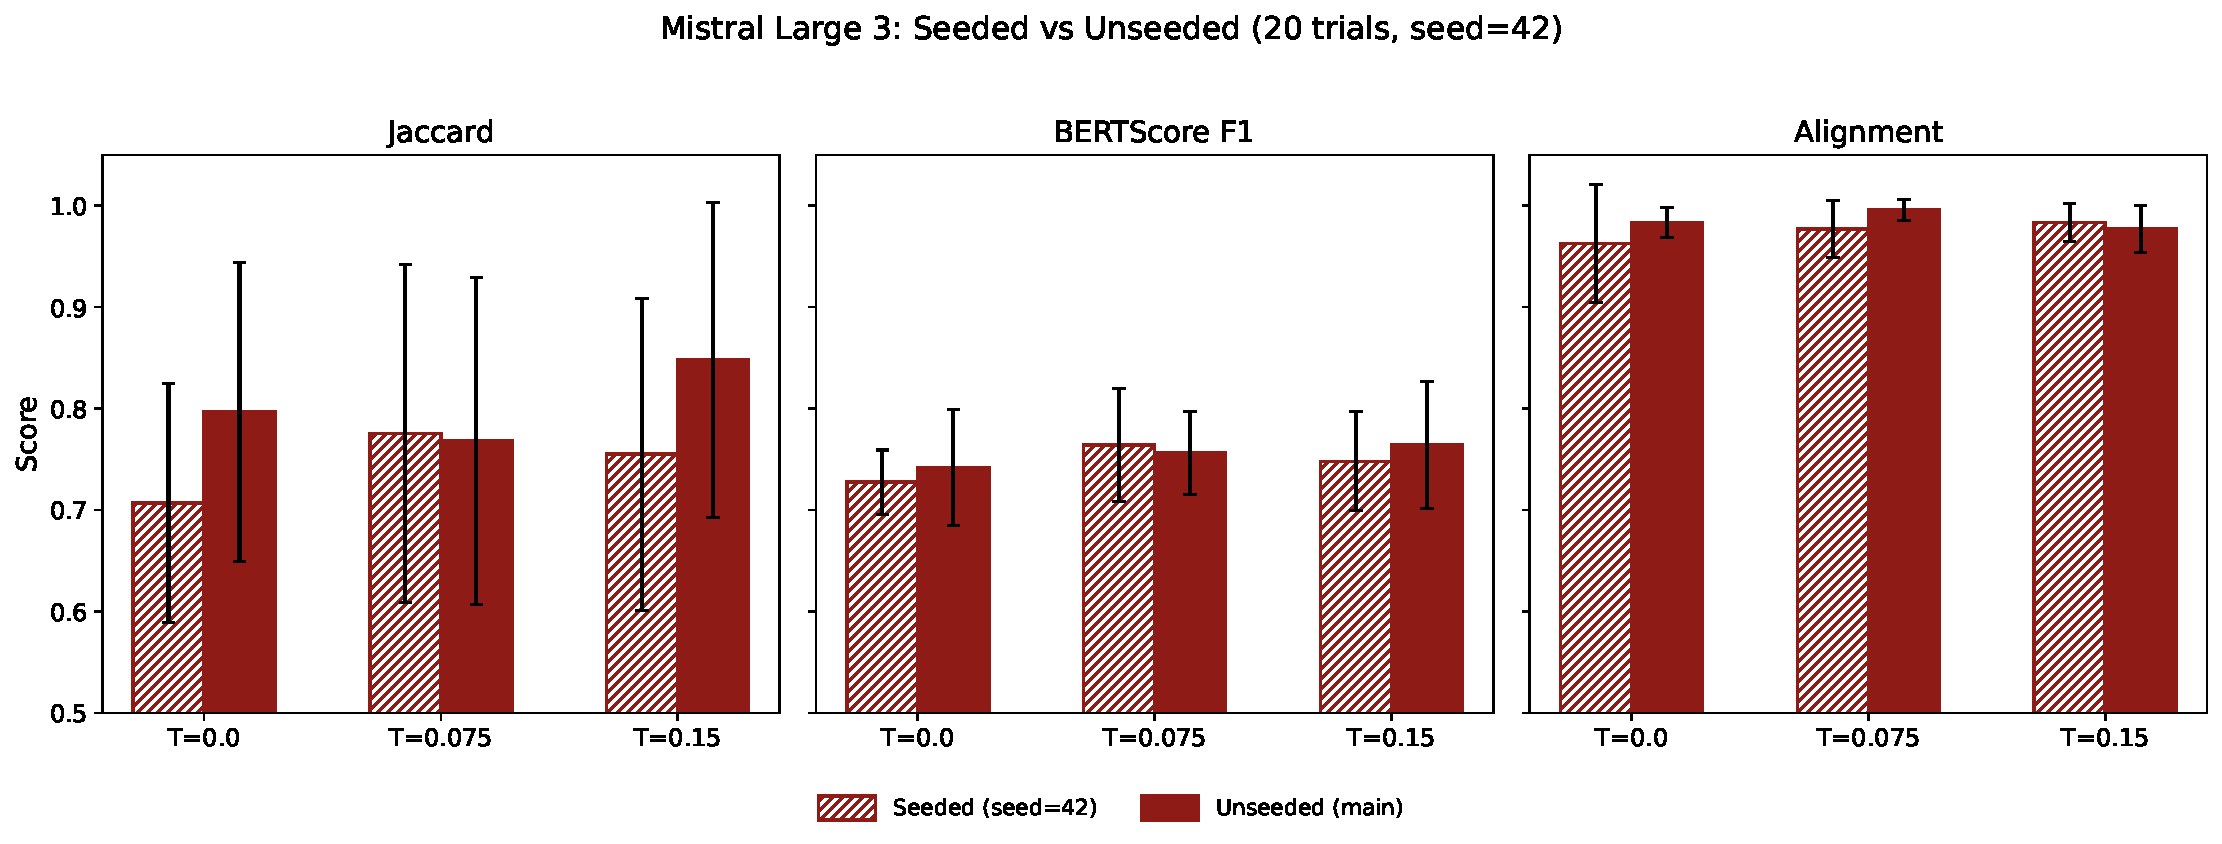
\includegraphics[width=.85\linewidth]{fig_seed_comparison}
  \caption{Seeded (\texttt{seed=42}) versus unseeded runs for Mistral Large~3. A fixed seed does not improve run-to-run consistency.}
  \label{fig:seed}
\end{figure}

\clearpage

\section{Models and Configurations Outside the Sweep}
\label{app:excluded}

The protocol needs two controls on the serving side: a temperature that reaches the model and a reasoning mode that can be switched off. Newer frontier models increasingly offer neither. Table~\ref{tab:excluded} records the cases met during this study, each re-probed on 2026-11-10 with single requests.

\begin{table}[h]
  \centering
  \small
  \begin{tabular}{llll}
    \toprule
    Model & Route & Request & Result \\
    \midrule
    GPT-5.4 & OpenRouter & $T{=}0.6$, effort \texttt{none} & 200, temperature dropped \\
    GPT-5.4 & OpenRouter, strict & $T{=}0.6$, effort \texttt{none} & 404, no endpoint \\
    GPT-5.4 & OpenRouter & $T{=}0.6$, effort \texttt{high} & 200, temperature dropped \\
    GPT-5.4 & OpenAI & $T{=}0.6$, effort \texttt{none} & 200 \\
    GPT-5.4 & OpenAI & $T{=}0.6$, effort \texttt{high} & 400, default temperature only \\
    GPT-6.1 Terra & OpenRouter & $T{=}0.6$, effort \texttt{none} & 200, temperature dropped \\
    GPT-6.1 Terra & OpenRouter, strict & $T{=}0.6$, effort \texttt{none} & 404, no endpoint \\
    GPT-6.1 Terra & OpenAI & $T{=}0.6$, effort \texttt{none} & 200 \\
    Claude Sonnet 4.6 & OpenRouter, strict & $T{=}0.6$ & 200 \\
    Opus 4.7 to Sonnet 5.5 & OpenRouter & $T{=}0.6$ & 200, temperature dropped \\
    Opus 4.7 to Sonnet 5.5 & OpenRouter, strict & $T{=}0.6$ & 404, no endpoint \\
    Claude Sonnet 5.5 & OpenRouter & $T{=}0.6$, effort \texttt{none} & 400, reasoning mandatory \\
    Mistral Large 4 & Mistral & effort \texttt{none} & 400, unsupported value \\
    Mistral Large 4 & OpenRouter & effort \texttt{none} & 400, unsupported value \\
    Mistral Large 4 & Mistral & effort \texttt{low} & 200, reasoning tokens returned \\
    \bottomrule
  \end{tabular}
  \caption{Parameter probes of 2026-11-10. ``Strict'' adds \texttt{require\_parameters}, under which OpenRouter refuses a request instead of dropping a parameter the endpoint does not support.}
  \label{tab:excluded}
\end{table}

The gateway behaviour that invalidated the first GPT-5.4 collection is unchanged. OpenRouter still answers a GPT-5.4 request that carries a temperature, and it also answers when the temperature is combined with high reasoning effort, a combination the OpenAI API itself rejects. The parameter is therefore removed before the request reaches the model. The native API accepts temperature at reasoning effort \texttt{none}, for GPT-5.4 and for the newer GPT-6.1 Terra alike, so later OpenAI models remain sweepable by the direct route. They are absent from this study because the proprietary pair was fixed in March 2026 (Section~\ref{sec:models}).

Anthropic models after Sonnet~4.6 are excluded for a different reason. Their API returns an error when a temperature is set \citep{anthropic2026sonnet5}, and the two 5.5 models can no longer switch reasoning off completely, so neither control is available. Through OpenRouter, the six Opus and Sonnet models released since then (Opus~4.7, 4.8, 5 and 5.5, Sonnet~5 and 5.5) all show the GPT pattern: the request with a temperature succeeds and the strict request fails. Sonnet~4.6 passes both.

Mistral Large~4 is the one case that was collected before the control disappeared. The public preview accepted reasoning effort \texttt{none}. The released model accepts only \texttt{low}, \texttt{medium} and \texttt{high} \citep{mistral2026reasoning}, rejects \texttt{none} on both routes, and reasons at \texttt{low}. Its preview results are therefore kept out of the model set and reported in Appendix~\ref{app:large4}.

\section{Mistral Large~4 Preview}
\label{app:large4}

Mistral Large~4 (1.05T MoE with 52B active parameters) was released as a public preview on 2026-10-06. It was collected on 2026-10-22, seven months after the main set, on the identical frozen histories and with a single registry entry plus one line that pins the base endpoint and excludes the zero-data-retention and EU variants. All 600 trials ran at reasoning effort \texttt{none} under the pinned regime, with the provider logged per trial and completion-token counts that match the visible output. The collection took 1\,h\,20\,min including re-runs after upstream rate limits. The weights followed on 2026-10-29 under the Mistral Ecosystem Open-Weight License, and the released model no longer accepts \texttt{none} (Appendix~\ref{app:excluded}). The measured configuration can no longer be requested, so Large~4 is not part of the model set and enters none of the statistics in Section~\ref{sec:results}. Table~\ref{tab:large4} reports what the preview showed.

\begin{table}[h]
  \centering\small
  \begin{tabular}{lrrrrr}
    \toprule
    Metric & $T{=}0.0$ & $T{=}0.075$ & $T{=}0.15$ & $T{=}0.3$ & $T{=}0.6$ \\
    \midrule
    Median Jaccard & 1.000 & 1.000 & 1.000 & 1.000 & 0.854 \\
    Mean Jaccard & 0.956 & 0.930 & 0.931 & 0.889 & 0.818 \\
    Modal-set agreement & 0.958 & 0.908 & 0.917 & 0.867 & 0.808 \\
    Mean BERTScore F1 & 0.794 & 0.771 & 0.751 & 0.720 & 0.691 \\
    Mean alignment & 0.954 & 0.952 & 0.971 & 0.969 & 0.969 \\
    \bottomrule
  \end{tabular}
  \caption{Mistral Large~4 preview by temperature (six vignettes per cell, 20 trials each).}
  \label{tab:large4}
\end{table}

Plan validity is 100\% and no trial failed with a judge error. Pooled median Jaccard is 1.000, modal-set agreement is 0.892, one strategy set covers all 20 trials in 19 of 30 conditions, mean BERTScore is 0.746, and mean alignment is 0.963. Large~4 shows no low-temperature optimum: mean Jaccard is highest at $T{=}0.0$ and falls to 0.818 at $T{=}0.6$, a trend that is not significant ($\rho=-0.31$, $p=.095$). The ceiling median comes with a narrower repertoire than any model in the set (77\% of 1{,}200 picks in the top two categories against 73\% for OLMo~3.1~32B, and no confrontation at all), so part of it is distributional (Section~\ref{sec:validity}). The remaining instability sits mostly in one vignette (avoidant, median 0.653).

Set next to the model set, Large~4 would share the median ceiling of 1.000 but trail Mistral Medium~3.5 on modal-set agreement (0.892 against 0.972) and response similarity (0.746 against 0.816). The comparison is cross-regime, seven months of serving changes lie in between, and the open-weight release may not behave like the measured checkpoint. It gives no reason to revise the recommendation for Medium~3.5 (Section~\ref{sec:sovereign-deployment}).

\section{Per-Condition Results}
\label{app:tables}

\begin{table}[H]
  \centering\small
  \begin{tabular}{lrrrrr}
    \toprule
    Model & $T{=}0.0$ & $T{=}0.075$ & $T{=}0.15$ & $T{=}0.3$ & $T{=}0.6$ \\
    \midrule
    Mistral Small 3.2 & 0.967 & 1.000 & 0.967 & 0.967 & 0.872 \\
    Mistral Small 4 & 0.746 & 0.874 & 0.935 & 0.646 & 0.625 \\
    Mistral Medium 3.5 & 1.000 & 1.000 & 1.000 & 1.000 & 0.967 \\
    Mistral Large 3 & 0.772 & 0.709 & 0.877 & 0.775 & 0.712 \\
    Mistral Large 4 & 1.000 & 1.000 & 1.000 & 1.000 & 0.854 \\
    Qwen 3.5 27B & 0.760 & 0.754 & 0.768 & 0.595 & 0.518 \\
    Qwen 3.5 122B & 1.000 & 1.000 & 0.967 & 0.853 & 0.730 \\
    Qwen 3.5 397B & 0.799 & 0.737 & 0.775 & 0.642 & 0.626 \\
    OLMo 3.1 32B & 1.000 & 1.000 & 0.911 & 0.911 & 0.746 \\
    Llama 3.3 70B & 0.705 & 0.730 & 0.732 & 0.668 & 0.597 \\
    Command A & 0.911 & 0.793 & 0.950 & 0.714 & 0.724 \\
    GPT-5.4 & 1.000 & 1.000 & 1.000 & 1.000 & 1.000 \\
    Claude Sonnet 4.6 & 0.868 & 0.779 & 1.000 & 0.854 & 0.933 \\
    \bottomrule
  \end{tabular}
  \caption{Median pairwise Jaccard per model and temperature (across 6 vignettes).}
\end{table}

\begin{table}[H]
  \centering\small
  \begin{tabular}{lrrrrr}
    \toprule
    Model & $T{=}0.0$ & $T{=}0.075$ & $T{=}0.15$ & $T{=}0.3$ & $T{=}0.6$ \\
    \midrule
    Mistral Small 3.2 & 0.757 & 0.766 & 0.758 & 0.743 & 0.708 \\
    Mistral Small 4 & 0.692 & 0.725 & 0.726 & 0.684 & 0.657 \\
    Mistral Medium 3.5 & 0.830 & 0.886 & 0.824 & 0.785 & 0.754 \\
    Mistral Large 3 & 0.742 & 0.756 & 0.764 & 0.743 & 0.705 \\
    Mistral Large 4 & 0.794 & 0.771 & 0.751 & 0.720 & 0.691 \\
    Qwen 3.5 27B & 0.831 & 0.780 & 0.754 & 0.715 & 0.687 \\
    Qwen 3.5 122B & 0.882 & 0.840 & 0.789 & 0.743 & 0.710 \\
    Qwen 3.5 397B & 0.750 & 0.759 & 0.735 & 0.726 & 0.717 \\
    OLMo 3.1 32B & 0.941 & 0.813 & 0.760 & 0.730 & 0.699 \\
    Llama 3.3 70B & 0.746 & 0.749 & 0.740 & 0.731 & 0.702 \\
    Command A & 0.771 & 0.762 & 0.754 & 0.700 & 0.690 \\
    GPT-5.4 & 0.770 & 0.762 & 0.760 & 0.751 & 0.745 \\
    Claude Sonnet 4.6 & 0.844 & 0.801 & 0.799 & 0.771 & 0.743 \\
    \bottomrule
  \end{tabular}
  \caption{Mean pairwise BERTScore F1 per model and temperature (across 6 vignettes).}
\end{table}

\begin{table}[H]
  \centering\small
  \begin{tabular}{lrrrrr}
    \toprule
    Model & $T{=}0.0$ & $T{=}0.075$ & $T{=}0.15$ & $T{=}0.3$ & $T{=}0.6$ \\
    \midrule
    Mistral Small 3.2 & 0.908 & 0.925 & 0.908 & 0.921 & 0.921 \\
    Mistral Small 4 & 0.837 & 0.842 & 0.790 & 0.806 & 0.776 \\
    Mistral Medium 3.5 & 0.965 & 0.944 & 0.960 & 0.963 & 0.975 \\
    Mistral Large 3 & 0.983 & 0.996 & 0.977 & 0.967 & 0.973 \\
    Mistral Large 4 & 0.954 & 0.952 & 0.971 & 0.969 & 0.969 \\
    Qwen 3.5 27B & 0.965 & 0.954 & 0.923 & 0.927 & 0.960 \\
    Qwen 3.5 122B & 0.983 & 0.973 & 0.979 & 0.983 & 0.969 \\
    Qwen 3.5 397B & 0.994 & 0.977 & 0.994 & 0.996 & 0.994 \\
    OLMo 3.1 32B & 0.898 & 0.917 & 0.910 & 0.915 & 0.894 \\
    Llama 3.3 70B & 0.919 & 0.890 & 0.888 & 0.875 & 0.875 \\
    Command A & 0.915 & 0.911 & 0.910 & 0.895 & 0.887 \\
    GPT-5.4 & 1.000 & 1.000 & 0.998 & 1.000 & 1.000 \\
    Claude Sonnet 4.6 & 1.000 & 1.000 & 1.000 & 1.000 & 0.998 \\
    \bottomrule
  \end{tabular}
  \caption{Mean plan--response alignment per model and temperature (across 6 vignettes).}
\end{table}

